\chapter{Sichtprüfung}
\label{ch:sichtpruefung}
% Verantwortlich: Person 3

Die Sichtprüfung beurteilt das Bauteil an der Prüfposition anhand von drei Merkmalen auf
seiner Seitenfläche: Sie liest die aufgeklebte Seriennummer, bestimmt den Durchmesser des
Durchgangslochs und prüft, ob die Kerbe vorhanden ist. Aus diesen Merkmalen entscheidet sie,
ob ein Gut- oder ein Schlechtteil vorliegt, und gibt das Ergebnis als
\texttt{InspectionResult} an den Orchestrator zurück (\cref{sec:schnittstellen}).

Wie die Objekterkennung ist auch die Sichtprüfung in eine reine Bildverarbeitung und den
Kamerazugriff getrennt, sodass sie sich mit gespeicherten Bildern testen lässt
(\cref{sec:teststrategie}). \Cref{fig:m3-kette} zeigt den Ablauf.

\begin{figure}[htbp]
  \centering
  \begin{tikzpicture}[
      box/.style={draw, rounded corners, align=center, minimum height=11mm, text width=28mm, font=\small},
      arr/.style={-{Stealth[length=2.2mm]}, thick},
      node distance=5mm and 7mm]
    \node[box] (img) {Bild der\\Seitenkamera};
    \node[box, right=of img] (loc) {Bauteil lokalisieren,\\Maßstab bestimmen};
    \node[box, right=of loc, yshift=15mm] (ocr) {Seriennummer\\(\acs{ocr})};
    \node[box, right=of loc] (hole) {Lochdurchmesser};
    \node[box, right=of loc, yshift=-15mm] (notch) {Kerbe};
    \node[box, right=of hole] (dec) {Gut-/Schlecht-\\Entscheidung};
    \draw[arr] (img) -- (loc);
    \draw[arr] (loc.east) -- ++(4mm,0) |- (ocr.west);
    \draw[arr] (loc) -- (hole);
    \draw[arr] (loc.east) -- ++(4mm,0) |- (notch.west);
    \draw[arr] (ocr.east) -- ++(4mm,0) |- (dec.west);
    \draw[arr] (hole) -- (dec);
    \draw[arr] (notch.east) -- ++(4mm,0) |- (dec.west);
  \end{tikzpicture}
  \caption{Ablauf der Sichtprüfung. Die drei Merkmale werden unabhängig voneinander bestimmt
           und gemeinsam bewertet.}
  \label{fig:m3-kette}
\end{figure}

% ------------------------------------------------------------------------------
\section{Aufbau der Prüfstation}
\label{sec:m3-aufbau}

Die Seitenkamera, eine \ac{usb}-Kamera, ist fest neben der Prüfposition montiert; die
bisherigen Testbilder haben $3840 \times 2160$~Pixel. Sie blickt möglichst senkrecht auf die
Seitenfläche des Bauteils, da eine schräge Ansicht die Längen im Bild perspektivisch verzerren
würde. Das Bauteil liegt auf einer 3D-gedruckten Prüfvorrichtung, deren Auflage
\SI{38}{\milli\metre} über der Platte liegt (\cref{fig:m3-vorrichtung}). Ein Halter an der
Vorrichtung legt den Abstand der Kamera zum Bauteil fest, und ein Hintergrund hinter dem
Bauteil sorgt dafür, dass sich das Loch deutlich von der Seitenfläche abhebt. Das Bauteil wird
nicht formschlüssig geführt; seine Lage ergibt sich aus der Ablegepose des Roboters. Während
der Prüfung wartet der Roboter über der Vorrichtung, sodass der Greifer nicht im Bild ist
(\cref{sec:m2-sequenz}).

\begin{figure}[htbp]
  \centering
  \missingfigure[figwidth=0.9\textwidth]{Prüfvorrichtung als CAD-Ansicht oder Foto: erhöhte
  Ablagefläche mit Bauteil, Kamerahalter mit Seitenkamera und Hintergrund hinter dem Bauteil.}
  \caption{Prüfvorrichtung mit Seitenkamera}
  \label{fig:m3-vorrichtung}
\end{figure}

Da die Objekterkennung die Orientierung über die Fase eindeutig bestimmt (\cref{sec:m1-pose})
und der Roboter das Bauteil immer in derselben Lage relativ zum Greifer aufnimmt, liegt es an
der Prüfposition stets gleich orientiert, mit Etikett, Loch und Kerbe zur Kamera. Wird die Fase
nicht gefunden, ist die Orientierung nur bis auf \ang{180} bestimmt; das Bauteil kann dann
verdreht liegen, und die Prüfmerkmale zeigen von der Kamera weg. Die Objekterkennung meldet
diesen Fall mit einer verringerten Konfidenz.

\begin{figure}[htbp]
  \centering
  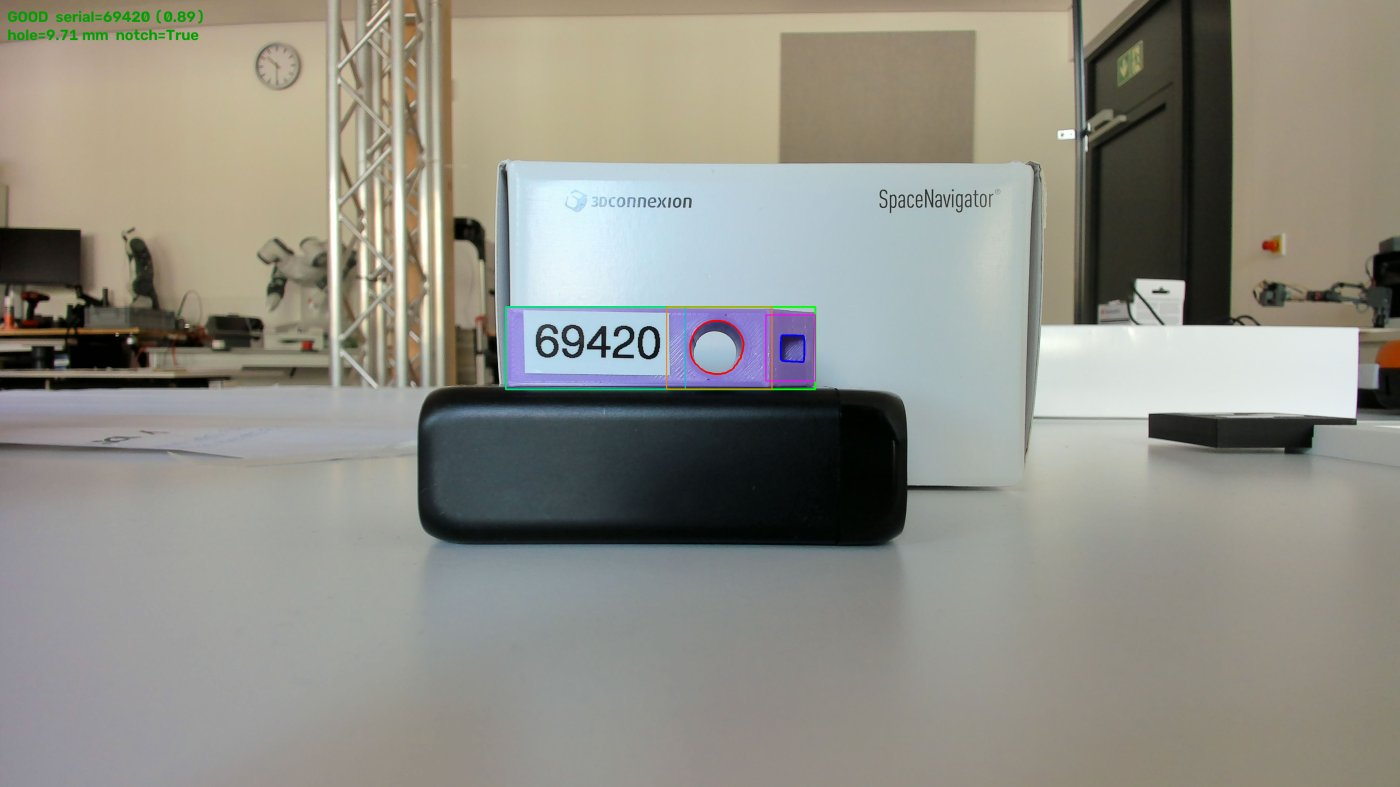
\includegraphics[width=\textwidth]{m3/m3_14_result.jpg}
  \caption{Seitenansicht eines Testbilds mit dem Ergebnis der Sichtprüfung: Bauteil-Box (grün),
  Prüfbereiche für Etikett, Loch und Kerbe, angepasste Ellipse am Loch (rot) und erkannte
  Kerbe (blau). Oben links das Urteil mit Seriennummer, Lochdurchmesser und Kerbe.}
  \label{fig:m3-rois}
\end{figure}

\todo[inline]{Kameramodell, Abstand und Beleuchtung der Prüfstation ergänzen.}

% ------------------------------------------------------------------------------
\section{Lokalisierung des Bauteils und Maßstab}
\label{sec:m3-lokalisierung}

Zuerst wird das Bauteil im Bild gesucht. Da es sich farblich deutlich vom Hintergrund
abhebt, geschieht das über eine Farbschwelle im \ac{hsv}-Farbraum (\cref{sec:farbraeume}):
Pixel mit dem Farbton des Bauteils und ausreichender Sättigung und Helligkeit gehören zum
Bauteil. Das weiße Etikett, das Loch und die Kerbe haben nicht die Farbe des Bauteils und
erscheinen in der Maske zunächst als Lücken. Ein morphologisches Schließen mit einem
Strukturelement in der Höhe des Bauteils füllt diese Lücken, sodass das umschließende
Rechteck die gesamte Seitenfläche erfasst.

Die drei Prüfbereiche (\ac{roi}) für Etikett, Loch und Kerbe sind relativ zu diesem Rechteck
festgelegt, jeweils als Bruchteil von dessen Breite und Höhe. Sie passen sich damit
automatisch an, wenn das Bauteil etwas näher an der Kamera oder etwas versetzt liegt.

Für die Umrechnung von Pixeln in Millimeter wird die sichtbare Höhe des Bauteils als Maßstab
verwendet: Da die tatsächliche Bauteilhöhe bekannt ist, ergibt ihr Verhältnis zur Höhe des
Rechtecks in Pixeln den Maßstab in Millimetern pro Pixel. Eine separate Kalibrierung mit
einer Messplatte ist dadurch nicht nötig, und der Maßstab bleibt auch bei kleinen
Abstandsänderungen richtig. Voraussetzung ist, dass Seitenfläche und Kamera annähernd
parallel stehen.

% ------------------------------------------------------------------------------
\section{Auslesen der Seriennummer}
\label{sec:m3-ocr}

Die Seriennummer ist eine fünfstellige Zahl auf dem Etikett. Sie wird mit EasyOCR
gelesen~\cite{easyocr}, einer lernbasierten \ac{ocr}-Bibliothek, die ohne separate
Installation einer \ac{ocr}-Software auskommt (\cref{sec:ocr}). Tesseract~\cite{smith2007}
wäre eine Alternative gewesen.

Der Etikettbereich wird ausgeschnitten und bei geringer Höhe vergrößert, da die
Texterkennung auf sehr kleine Schrift schlechter anspricht. Die Erkennung ist auf Ziffern
beschränkt. Aus den erkannten Textkandidaten wird derjenige mit der höchsten Konfidenz
gewählt, der dem erwarteten Format entspricht; das Format ist als regulärer Ausdruck für
genau fünf Ziffern in der Konfiguration hinterlegt. Liegt die Konfidenz unter einer
Mindestschwelle, gilt die Seriennummer als nicht lesbar.

% ------------------------------------------------------------------------------
\section{Vermessung des Lochdurchmessers}
\label{sec:m3-loch}

Im Lochbereich ist die Seitenfläche des Bauteils hell und farbig. Das Loch hebt sich davon ab,
allerdings je nach Beleuchtung unterschiedlich: Die Bohrungswand erscheint dunkel, durch das
Loch hindurch kann aber auch heller Hintergrund sichtbar sein. Deshalb wird nicht nach einer
bestimmten Farbe des Lochs gesucht, sondern nach allem, was nicht zur hellen Seitenfläche
gehört. Als Referenz für die Helligkeit der Fläche dient ein hohes Perzentil der
bauteilfarbenen Pixel im Bereich.

Die so gefundenen Regionen werden morphologisch bereinigt und auf eine Mindestgröße gefiltert.
Für jede Region wird ihre Rundheit bestimmt, also das Verhältnis ihrer Fläche zur Fläche des
kleinsten umschließenden Kreises. Die rundeste Region ist das Loch, sofern ihre Rundheit eine
Mindestschwelle überschreitet. An ihre Kontur wird eine Ellipse nach der Methode der
kleinsten Quadrate angepasst (\cref{sec:messtechnik}); der Mittelwert der beiden Achsenlängen
ergibt den Durchmesser in Pixeln, der mit dem Maßstab aus \cref{sec:m3-lokalisierung} in
Millimeter umgerechnet wird. Die Ellipse berücksichtigt, dass ein kreisrundes Loch bei leicht
schräger Ansicht elliptisch erscheint. Eine Kreisdetektion mit der Hough-Transformation
(\cref{sec:messtechnik}) wäre möglich, liefert den Radius aber nur in der Auflösung ihres
Akkumulators, während der Ellipsen-Fit alle Konturpunkte nutzt.

% ------------------------------------------------------------------------------
\section{Prüfung auf Kerbe}
\label{sec:m3-kerbe}

Die Kerbe ist eine kleine rechteckige Öffnung am Rand der Seitenfläche. Je nach Licht ist sie
dunkler als die Fläche, anders gefärbt oder nur an ihren Kanten zu erkennen. Deshalb werden
Kandidaten auf zwei Wegen gesucht:
\begin{itemize}
  \item \textbf{Regionenbasiert:} Pixel, die deutlich dunkler oder deutlich anders gesättigt
        sind als die umgebende Fläche. Die Referenz für die Fläche ist der Median am Rand des
        Kerbenbereichs.
  \item \textbf{Kantenbasiert:} geschlossene Kantenzüge aus einer Kantendetektion, für den Fall,
        dass die Öffnung dieselbe Farbe wie die Fläche hat und sich nur durch ihre Ränder
        abzeichnet.
\end{itemize}

Aus allen Kandidaten werden nur solche betrachtet, die vollständig im Kerbenbereich liegen,
eine plausible Größe haben und annähernd quadratisch bis mäßig länglich sind. Für jeden wird
die Rechteckigkeit bestimmt, also das Verhältnis seiner Fläche zur Fläche des kleinsten
umschließenden Rechtecks. Überschreitet der rechteckigste Kandidat eine Mindestschwelle, gilt
die Kerbe als vorhanden. Ein Template-Matching gegen ein Referenzbild der Kerbe
(\cref{sec:messtechnik}) wäre eine Alternative, reagiert aber im Allgemeinen empfindlicher
auf Änderungen von Beleuchtung und Lage.

% ------------------------------------------------------------------------------
\section{Gut-/Schlecht-Entscheidung}
\label{sec:m3-entscheidung}

Ein Bauteil ist ein Gutteil, wenn alle drei Merkmale erfüllt sind: Die Seriennummer ist
lesbar und entspricht dem Format, das Loch wurde gefunden und sein Durchmesser liegt innerhalb
der Toleranz um den Sollwert, und die Kerbe ist vorhanden. Andernfalls ist es ein Schlechtteil,
und jeder nicht erfüllte Punkt wird als Grund im Prüfergebnis festgehalten
(\cref{fig:m3-entscheidung}). Die Toleranz des Lochdurchmessers dient der Demonstration und
entspricht keiner Fertigungsvorgabe.

\begin{figure}[htbp]
  \centering
  \begin{tikzpicture}[pap]
    \node[pap term] (start) {Seriennummer $s$, Lochdurchmesser $d$, Kerbe $k$};
    \node[pap proc, below=of start] (init) {Liste der Gründe $G$ leeren};
    \node[pap dec, below=of init] (d1) {Seriennummer lesbar\\und im Format?};
    \node[pap dec, below=9mm of d1] (d2) {Loch gefunden?};
    \node[pap dec, below=of d2] (d3) {$|d - d_\text{soll}| \le \Delta d$\,?};
    \node[pap dec, below=9mm of d3] (d4) {Kerbe vorhanden?};
    \node[pap dec, below=9mm of d4] (d5) {$G$ leer?};
    \node[pap good, below=of d5] (gut) {Gutteil};
    \node[pap bad, right=12mm of d5] (schlecht) {Schlechtteil\\mit Gründen $G$};
    \node[pap proc=36mm, right=10mm of d1] (r1) {Grund: Seriennummer ungültig};
    \node[pap proc=30mm, left=10mm of d2] (r2) {Grund: Loch nicht gefunden};
    \node[pap proc=36mm, right=10mm of d3] (r3) {Grund: Durchmesser außerhalb der Toleranz};
    \node[pap proc=36mm, right=10mm of d4] (r4) {Grund: Kerbe fehlt};
    \coordinate (j1) at ($(d1.south)!0.5!(d2.north)$);
    \coordinate (j3) at ($(d3.south)!0.5!(d4.north)$);
    \coordinate (j4) at ($(d4.south)!0.5!(d5.north)$);
    \draw[pap arr] (start) -- (init);
    \draw[pap arr] (init) -- (d1);
    \draw[pap arr] (d1) -- node[pap lbl, right=1pt, pos=0.3] {ja} (d2);
    \draw[pap arr] (d2) -- node[pap lbl, right=1pt] {ja} (d3);
    \draw[pap arr] (d3) -- node[pap lbl, right=1pt, pos=0.3] {ja} (d4);
    \draw[pap arr] (d4) -- node[pap lbl, right=1pt, pos=0.3] {ja} (d5);
    \draw[pap arr] (d5) -- node[pap lbl, right=1pt] {ja} (gut);
    \draw[pap arr] (d5) -- node[pap lbl] {nein} (schlecht);
    \draw[pap arr] (d1) -- node[pap lbl] {nein} (r1);
    \draw[pap arr] (d2) -- node[pap lbl] {nein} (r2);
    \draw[pap arr] (d3) -- node[pap lbl] {nein} (r3);
    \draw[pap arr] (d4) -- node[pap lbl] {nein} (r4);
    \draw[pap arr] (r1) |- (j1);
    \draw[pap arr] (r2) |- (j3);
    \draw[pap arr] (r3) |- (j3);
    \draw[pap arr] (r4) |- (j4);
  \end{tikzpicture}
  \caption{Gut-/Schlecht-Entscheidung. Jedes nicht erfüllte Merkmal wird als Grund in $G$
  festgehalten.}
  \label{fig:m3-entscheidung}
\end{figure}

Für das Testbauteil gelten eine Bauteilhöhe von \SI{15}{\milli\metre} als Maßstab, ein
Soll-Durchmesser des Lochs von \SI{10}{\milli\metre} und eine Toleranz von
\SI{\pm 0,4}{\milli\metre}. Die Toleranz ist ein Demonstrationswert und keine
Fertigungstoleranz.

% ------------------------------------------------------------------------------
\section{Zwischenfazit}

Auf vier Testbildern eines Gutteils wird die Seriennummer \enquote{69420} jedes Mal richtig
gelesen. Das Verhältnis von Lochdurchmesser zu Bauteilhöhe streut auf den ersten drei Bildern
um \SI{\pm 1,2}{\percent} (0,647; 0,663; 0,649), was etwa \SIrange{9.7}{9.9}{\milli\metre}
entspricht. Künstlich erzeugte Fehler, bei denen Kerbe oder Loch im Bild übermalt sind, werden
als Schlechtteil erkannt.

\todo[inline]{Nach den Versuchen ergänzen: Ergebnisse mit der Seitenkamera am Aufbau, echte
Fehlerteile, aufgetretene Probleme.}
